\chapter{Odometrie}
    L’odometrie désigne l’évaluation de la position du robot dans un repère fixe à l’aide de
    mesures sur son déplacement. On se place dans le cas d’une odométrie calculée à l’aide de deux codeurs incrémentaux à quadrature montés sur roue codeuses. On distingue roues motrices et roues codeuses : en effet, disposer les codeurs directement sur l’arbre moteur risque de provoquer des enregistrement de déplacements liés à un patinage des moteurs en cas de roue motrice bloquée. Les methodes d’odometrie liés à l’utilisation de capteurs optiques ne seront pas traités ici.

    \section{contexte}
        On échantillonne les impulsions des encodeurs périodiquement tous les $d\tau$ . On choisit l’origine au millieu de l’essieu du robot, et on assimile le robot à ce point. La position du robot est représentée par le vecteur
        \begin{equation}
            p = \begin{pmatrix}
                x\\
                y\\
                \theta
            \end{pmatrix}
        \end{equation}

        Avec:
        \begin{itemize}
            \item $(x, y)$ La position du millieu de l’essieu
            \item $\theta$ L'orientation du robot
        \end{itemize}

    \newpage
    \section{Interprétation des signaux}
        \subsection{Valeur et sens de rotation}
        \begin{figure}[h]
            \begin{center}
                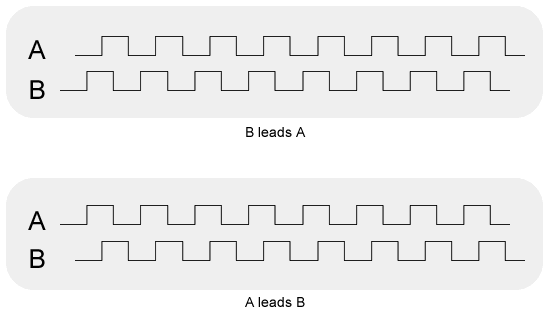
\includegraphics[scale=0.5]{encoder.png}
            \end{center}

            \caption{Signaux envoyés par un encodeur optique rotatif à quadrature}
        \end{figure}
        Chaque encodeur donne deux signaux : le signal A et le signal B. Chaque signal est déphasé de $\pi/4$, et le sens d’un signal peut être déduit de la valeur du deuxième signal au même moment.

        \textbf{Exemple} : l’écoute d’un front montant sur A peut être interpété comme une impulsion positive si l’état de B est à bas au même moment.\\
        On note :
        $$
            \begin{cases}
                impulsions_{gauche}\\
                impulsions_{droite}
            \end{cases}
        $$
        la \textit{somme algébrique des impulsions} depuis le dernier échantillonnage sur les roues gauche et droite.

        \subsubsection{Multiplication logicielle de la résolution}
            Il est possible de multiplier la résolution de son encodeur pour peu qu’il soit de bonne qualité, i.e que le rapport cyclique des signaux envoyés soit de 0.5. Notons que cette multipli-
            cation est purement logicielle, et que par conséquent elle induit une imprécision (bien qu’elle amène aussi une précision suplémentaire du au nombre d’impulsions plus important !).\\
            On peut ainsi doubler la résolution en comptant aussi bien les fronts montant que déscendant sur A, voir même quadrupler si on applique le même principe sur B.\\
            Dans le reste de ce document, on notera $C_r$ le coefficient de résolution, qui représente le nombre de fronts comptés par période du signal.

    \newpage
    \section{Formules de passage}
        On raisonnera la plupart du temps en impulsions d’encodeur et non en mètres. Voyons alors comment passer d’un système à un autre.\\
        On note :
        \begin{itemize}
            \item $impulsions_{parTour}$ le nombre d’impulsion d’encodeur par tour de roue codeuse.
            \item $impulsions_{codeur}$ le nombre d’impulsion d’un tour d’encodeur originel.
            \item $rapport_{reduction}$ le rapport de réduction entre le nombre de tour de roue codeuse et le nombre de tours d’encodeur.\\
        \end{itemize}

        On a la relation suivante :
        \begin{equation}
            impulsions_{parTour} = C_r \times rapport_{reduction} \times impulsion_{encodeur}
        \end{equation}
        Ainsi, pour passer de mètres en impulsions :
        \begin{equation}
            [m] = \frac{[impulsions] \times 2\pi \times R}{impulsions_{parTour}}
        \end{equation}

        \subsubsection{En pratique}
            On utilise le fait que la relation ci-dessus ne fait intervenir que des constantes.\\
            On peut donc la simplifier :
            \begin{equation}
                [m] = K_1 * [impulsions]
            \end{equation}
            Avec $K_1$ le facteur permettant de passer d’un système à l’autre. On le détermine alors empiriquement en faisant parcourir une distance $L$ en mètres au robot et on mesure la distance $\rho$ en impulsions parcourue. On trouve alors :
            \begin{equation}
                K_1 = \frac{L}{\rho}
            \end{equation}

    \newpage
    \section{Traitement des données}
        \begin{figure}[h]
            \begin{center}
                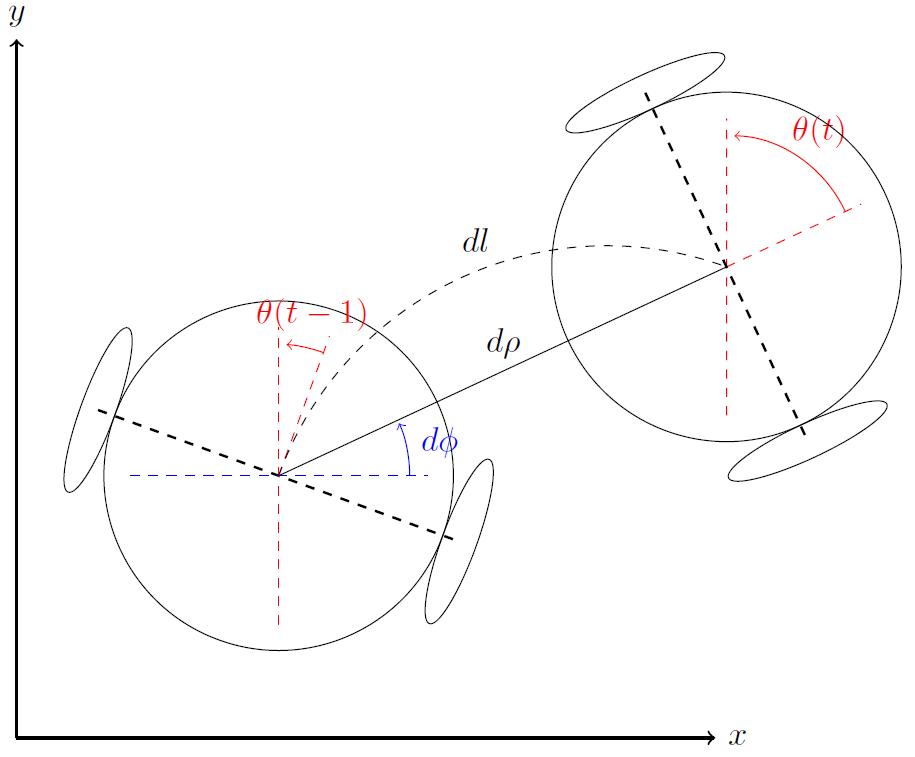
\includegraphics[scale=0.35]{odometry.png}
            \end{center}

            \caption{Evolution du système pendant $d\tau$}
        \end{figure}
        On fait une \textbf{approximation linéaire} sur le déplacement du robot, c’est à dire que l’on considère que sur un intervalle de temps $d\tau$ \textit{assez court} (en pratique 5ms semble suffisant), le déplacement dl du robot est une droite, i.e $d\rho$ = dl.\\
        De même, on consièdre que l’orientation de cette droite est la moyenne de l’orientation en début de déplacement et de l’orientation en fin de déplacement. On note alors $\phi$ l’angle de $d\rho$ :
        $$
            \phi = \frac{\theta(t) + \theta(t-1)}{2} = \theta(t-1)+ \frac{d\theta}{2}
        $$
        Au cours de $d\tau$ à l’instant t :
        \begin{equation}
            d\tau = \frac{impulsions_{gauche} + impulsions_{droite}}{2}
            \label{dTAU}
        \end{equation}
        \begin{equation}
            d\theta = \frac{impulsions_{gauche} - impulsions_{droite}}{entraxe}
            \label{dTHETA}
        \end{equation}
        Avec entraxe la distance entre le centre des deux roues codeuses.\\

        \textbf{En pratique} : Comme pour le facteur de passage entre ticks et mètres, la valeur de l’entraxe utilisée sur le système final doit être déterminée \textbf{empiriquement}. On fait alors tourner le robot sur $n\pi$ en sommant la différence de ticks. On trouve alors :
        \begin{equation}
            entraxe = \frac{\sum(impulsions_{gauche} - impulsions_{droite})}{n\pi}
        \end{equation}

        \newpage
        On procède à une intégration numérique\footnote{i.e une somme discrète, considérée continue car $d\tau$ est petit} pour obtenir l’orientation du robot dans le repère fixe:
        $$
            \theta(n) = \int_0^t d\theta
        $$
        Pour obtenir les coordonnées du robot dans le repère fixe, on projette la droite portée par $\rho$.
        \begin{equation}
            dx = d\rho \times cos(\theta(t-1) + \frac{d\theta}{2})
        \end{equation}
        \begin{equation}
            dy= d\tau \times sin(\theta(t-1) + \frac{d\theta}{2})
        \end{equation}
        A nouveaupar intégration numérique, on obtient les coordonnées du robot dans le repère fixe:
        $$ x(t) = \int_0^t dx $$
        $$ y(t) = \int_0^t dy $$
        Finalement, en notant $p$ la position du robot, on peut éxprimer $p'$ sa position après un échantillonnage.
        \begin{equation}
            p' =
            \begin{pmatrix}
                x\\
                y\\
                \theta
            \end{pmatrix} +
            \begin{pmatrix}
                \frac{impulsions_{gauche}+impoulsions_{droite}}{2}\times cos(\theta+\frac{impulsions_{gauche}-impulsions_{droite}}{2\times entraxe})\\
                \frac{impulsions_{gauche}+impoulsions_{droite}}{2}\times sin(\theta+\frac{impulsions_{gauche}-impulsions_{droite}}{2\times entraxe})\\
                \frac{impulsions_{gauche}-impulsions_{droite}}{entraxe}
            \end{pmatrix}
        \end{equation}

        \newpage
        \subsubsection{Code d'exemple}
            \begin{lstlisting}[language=JavaScript]
// Constantes theoriques
const REFRESH_TIME = 5; //ms
const RESOLUTION_COEF = 2;
const ENCODER_TICKS = 500;
const REDUCTOR_RATIO = 1.2;
const WHEEL_RADIUS = 0.06; //metres
const ENTRAXE = metersToTicks(0.5); //impulsions

let leftEncoder = new Encoder();
let rightEncoder = new Encoder();
let distance = 0;
let orientation = 0;
let x = 0;
let y = 0;
let lastCall = null;

function ticksToMeters(ticks) {
    return (ticks * 2 * Math.PI * WHEEL_RADIUS) /
        (RESOLUTION_COEF *REDUCTOR_RATIO * ENCODER_TICKS);
}

function metersToTicks(meters) {
    return (meters * RESOLUTION_COEF *REDUCTOR_RATIO * ENCODER_TICKS) /
        (2 * Math.PI * WHEEL_RADIUS);
}

/**
* Fonction de rafraichissement appelee le plus frequemment possible
*/
function compute() {
    let now = Date.now();
    // On s'assure que les calculs sont fait a intervalles reguliers
    if (now - previousOrientation >= REFRESH_TIME) {
        lastCall = now;
        let leftTicks = leftEncoder.getTicks();
        let rightTicks = leftEncoder.getTicks();
        leftEncoder.resetTicks();
        rightEncoder.resetTicks();
        let rho = (leftTicks + rightTicks) / 2;
        let dTheta = (leftTicks - rightTicks) / ENTRAXE;
        let dx = rho * Math.cos(orientation + dTheta / 2);
        let dy = rho * Math.sin(orientation + dTheta / 2);
        x += dx;
        y += dy;
        orientation += dTheta;
    }
}

function getRobotStatus() {
    return {
        x : ticksToMeters(x),
        y : ticksToMeters(y),
        orientation: orientation
    }
}
        \end{lstlisting}